%\documentclass{article}
%\usepackage{graphicx,subfigure}
%\begin{document}

\begin{figure}[!h]
  \centering
  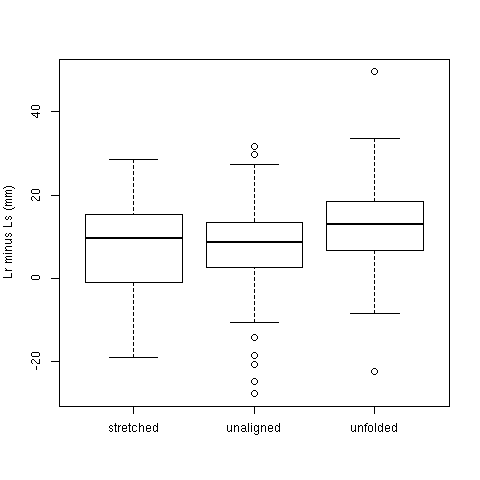
\includegraphics[width=1.0\textwidth]{figLrminusLs.png}
%   15fibreLrminusLs.png is original 
  \caption{Boxplot of relaxed fibre length minus staple length for fibres removed from staples for the SF technique, separately for each crimptype. There are 15 fibres per sheep, one staple per sheep and 21 sheep. The median values for each crimptype are stretched 9.56, unaligned 8.70, and unfolded 12.85.}
\label{fig:LrminusLs}
\end{figure}

%\end{document}

